
%(BEGIN_QUESTION)
% Copyright 2006, Tony R. Kuphaldt, released under the Creative Commons Attribution License (v 1.0)
% This means you may do almost anything with this work of mine, so long as you give me proper credit

Calculate the required valve $C_{v}$ rating to achieve a flow rate of 125 GPM, assuming that the nozzle at the end of the pipe drops a pressure of 30 PSID at that rate of flow.  Assume a liquid with a specific gravity of 0.85, and a pump suction (inlet) pressure of 0 PSIG at all times:

$$\includegraphics[width=15.5cm]{i01410x01.eps}$$

Also, calculate the approximate size of the valve (nominal pipe diameter, in inches) given a double-ported, contoured plug globe valve ($C_d = 13$).

\vskip 20pt \vbox{\hrule \hbox{\strut \vrule{} {\bf Suggestions for Socratic discussion} \vrule} \hrule}

\begin{itemize}
\item{} Suppose the pump were powered by an electric motor through a VFD (Variable Frequency Drive), allowing adjustment of pump speed.  How would a {\it decrease} in pump speed alter the pump curve, if at all?
\item{} What type of control valve and actuator are used in this application?
\item{} Does it matter where the control valve is installed in the vertical pipe section (e.g. at the top versus at the bottom versus in the middle)?  Explain why or why not.
\end{itemize}

\underbar{file i01410}
%(END_QUESTION)





%(BEGIN_ANSWER)

\noindent
{\bf Partial answer:}

\vskip 10pt

$C_{v}$ = 20.77
 
%(END_ANSWER)





%(BEGIN_NOTES)

Calculating flow capacity ($C_v$) of control valve:

$$\Delta P = 70 - \left(25 \hbox{ ft liquid} \over 1 \right)  \left(12 \hbox{ in} \over 1 \hbox{ ft}\right)  \left(1 \hbox{ PSI} \over 27.68 \hbox{ "WC}\right)  \left(0.85 \hbox{ "WC} \over 1 \hbox{ " liquid}\right) - 30 = 30.79 \hbox{ PSID}$$

$$Q = C_v \sqrt{\Delta P \over G_f}$$

$$C_v = {Q \over \sqrt{\Delta P \over G_f}}$$

$$C_v = {125 \over \sqrt{30.79 \over 0.85}} = 20.77$$

\vskip 10pt

Calculating pipe size of control valve:

$$C_d = {C_v \over d^2}$$

$$d^2 = {C_v \over C_d}$$

$$d = \sqrt{C_v \over C_d}$$

$$d = \sqrt{20.77 \over 13} = 1.264 \hbox{ inches}$$


\vskip 10pt

A 1.5 inch double-ported, contoured-plug globe valve would be just about right for this application.

%INDEX% Final Control Elements, pump: pressure/flow curve
%INDEX% Final Control Elements, valve: sizing

%(END_NOTES)


